\loesung{
\begin{center}
	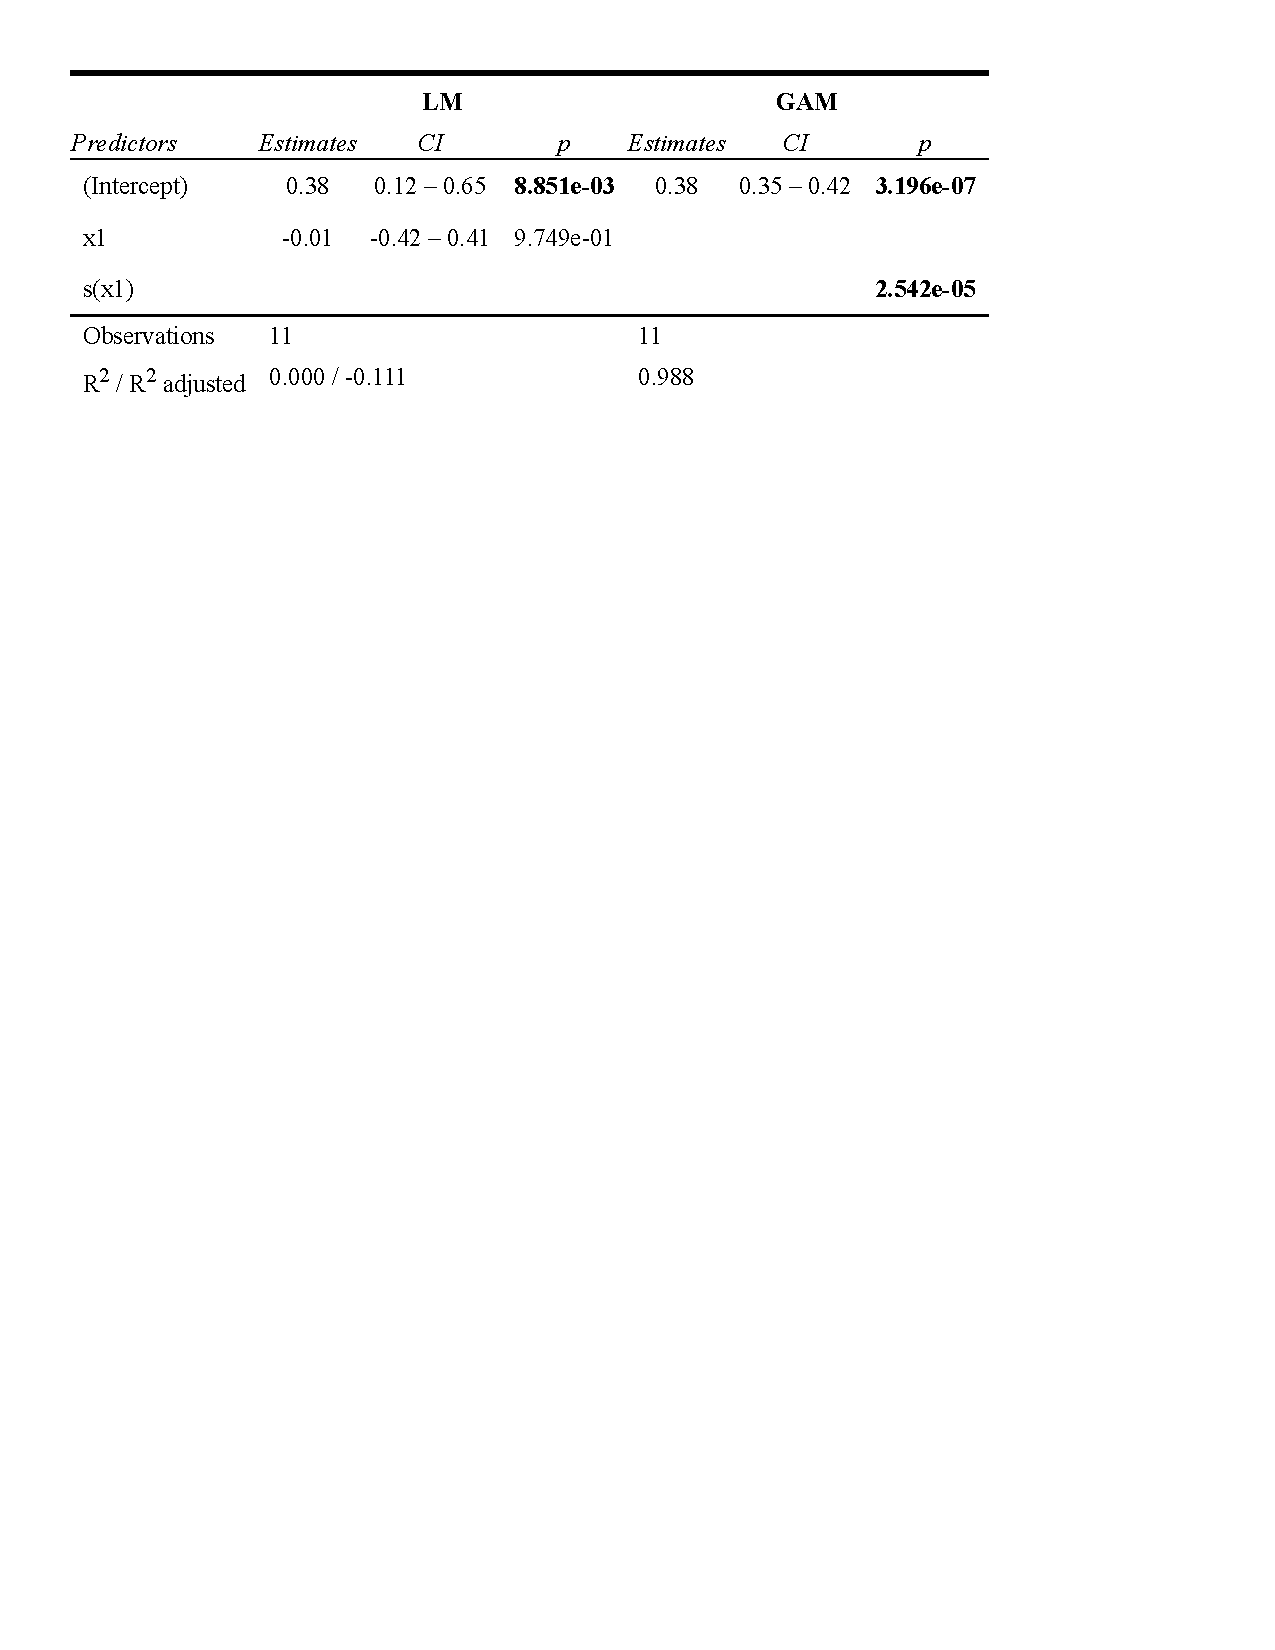
\includegraphics[clip, trim=0.5cm 21cm 5cm 1cm, width=.6\textwidth]{figure/GAM_LM_Output.pdf}
\end{center}
The R$^2-$value for the GAM model is the adjusted one.

\bigskip
\begin{enumerate}[a)]

    \item 
    What is the \textbf{Adjusted} $\mathbf{R^2}$? 
    
    Problem with normal $R^2$:  It rises each time a feature is added, no matter if the added feature improves the fit or not.
    
    The adjusted $R^2$ considers the number of terms in a model and only increases after adding a feature, if the fit becomes better:
    $$
    \text{adj. } R^2 = 1-\frac{SSE_{LM}\, / \, (n-p-1)}{SSE_{c}\, / \, (n-1)},  \qquad \text{but} \qquad R^2 = 1-\frac{SSE_{LM}}{SSE_{c}}
    $$
    where $n$ is the sample size and $p$ is the number of features.
    
    Hence, it is the proportion of explained variance using unbiased estimates for the variances.

    \textbf{Interpretation:}
    The very low values for $R^2$ for the linear model show that no variance can be explained by a linear model, so there is no linear relationship, whereas the high adjusted $R^2$ for the GAM shows that there is a strong relationship found by the GAM.

	\item LM: Since the $\beta$-values are not scaled, they are not well interpretable. From the high p-value, the large confidence intervals and $R^2$ = 0 (see above) it can be inferred that there is no linear relationship. (Remember: $R^2 = \rho^2$. )
	\item GAM: The p-value of $2.54 \times 10^{-5}$ (as the adjusted $R^2$ value) reveals that there is a strong relationship between $x_1$ and $x_2$. Hence, generalized additive models (GAM) are able to detect non-linear relationships. The p-value does not reveal the shape of this relationship, but we can visualize the relationship learned by the GAM incl. the confidence band, see figure \ref{fig:ex_sol_LM_vs_GAM_visualization}.
	% \begin{center}
	% 	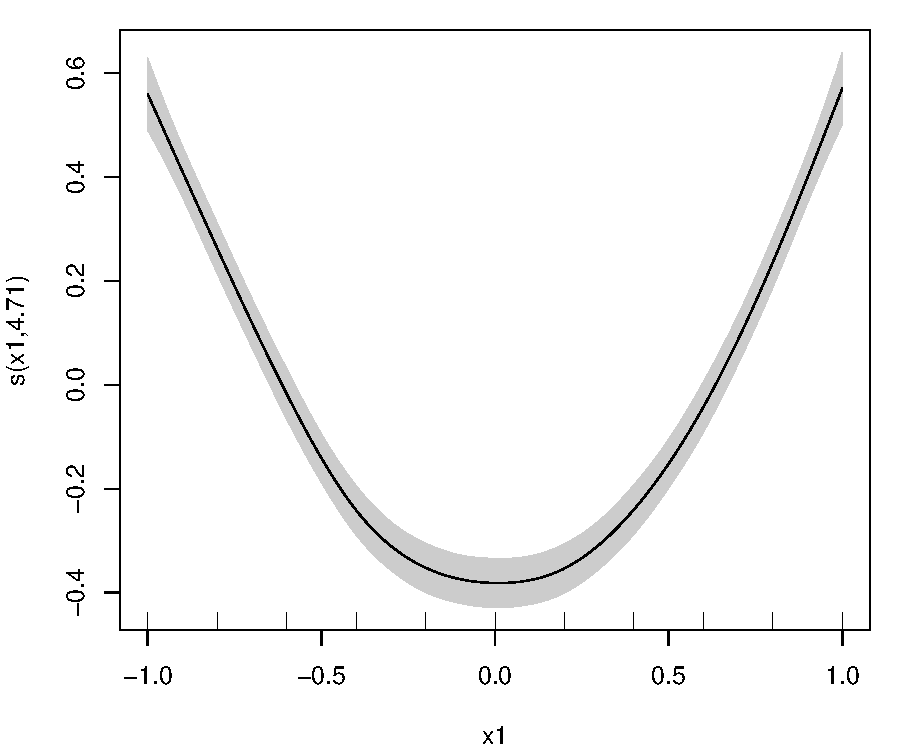
\includegraphics[width=.6\textwidth]{figure/gam.pdf}
	% \end{center}

    \begin{center}
    \begin{figure}[!ht]
        \vspace{-10pt} % Note that this is only to ensure a normal, not to big margin around the figure
        \centering
        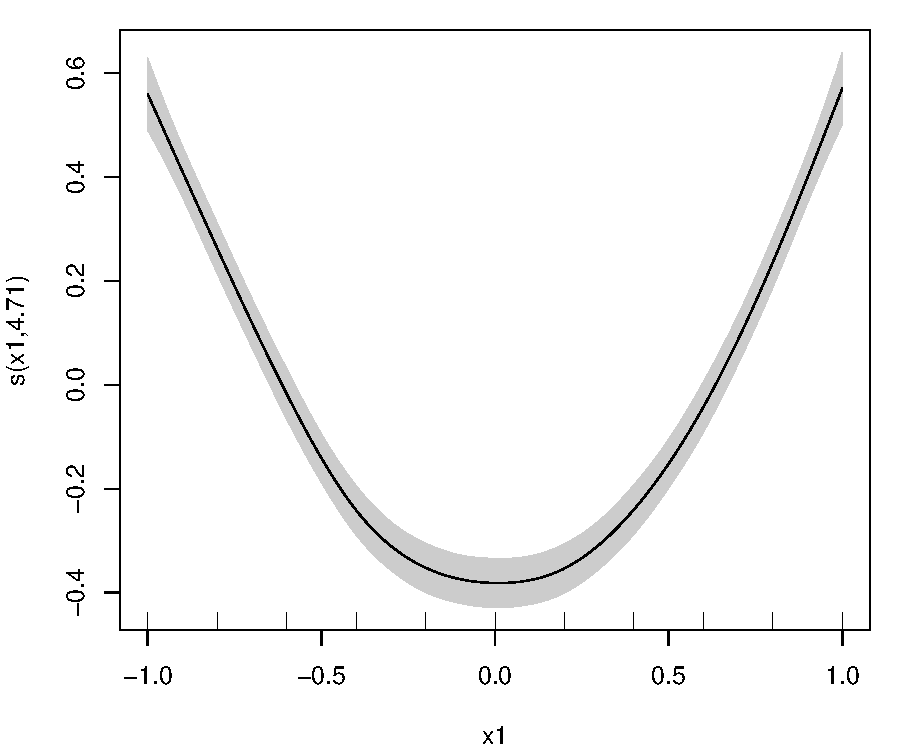
\includegraphics[width=.6\textwidth]{figure/gam.pdf}
        \vspace{-10pt}
        \caption{Visualization of the GAM output over a certain range, showing the relationship learned by the GAM}
        \label{fig:ex_sol_LM_vs_GAM_visualization}
    \end{figure}
    \end{center}
\end{enumerate}

}
